%!TEX root = ../these.tex

\chapter{
  Описание формата файлов DBS
}
\label{app:dbs}

DBS ---
унаследованный двоичный формат файла
обмена информацией в CAD-системах.
В данной диссертационной работе
используется в основном представление
геометрической информации о плоских деталях.

DBS-файл состоит из произвольного количества DBS-записей.
Каждая запись имеет тип, определяющий какие данные в ней содержатся.
Основные типы записей сведены в табл.~\ref{tab:dbs.records}.

\begin{table}[h]
  \caption{Основные виды DBS-записей}
  \label{tab:dbs.records}
  \centering
  \begin{tabular}{|r|l|}
    \hline
    Тип записи & Назначение \\
    \hline
    1  & Геометрия одного контура детали  \\
    2  & Копия контура (с геометрическим преобразованием) \\
    4  & Последовательность обработки \\
    5  & Текст  \\
    7  & Плоскость  \\
    8  & Объединение нескольких контуров в деталь \\
    9  & Фаска  \\
    10 & Револьверная головка \\
    11 & Токарный инструмент  \\
    12 & Инструментальный блок  \\
    13 & Приспособление \\
    21 & Фрезерный инструмент \\
    25 & Маркировка \\
    26 & Наименование детали  \\
    27 & Площадь и периметр детали  \\
    28 & Примечание \\
    \hline
  \end{tabular}
\end{table}

Для каждой записи указывается длина,
это позволяет пропускать неизвестные или
неинтересные типы записей,
читая только необходимые в данный момент.
Благодаря этому формат DBS
легко расширяем,
возможно создание новых типов записей
без необходимости изменять существующий
код импорта / экспорта.

Служебная информация в полях записей систематически дублируется,
что усложняет задачу корректной записи DBS-файла.

\section*{Заголовок записи}

Все записи
(кроме последней)
начинаются со стандартного заголовка,
содержащего длину, тип записи
и служебную информацию.

\newcommand{\dbsRecord}[1]{
  \noindent
  \begin{tabularx}{\textwidth}{|>{\raggedleft}p{3em}|>{\centering}p{4em}|>{\centering}p{3em}|X|}
    \hline
    \multicolumn{1}{|c|}{Смещение} &
    \multicolumn{1}{c|}{Тип}      &
    \multicolumn{1}{c|}{Имя}      &
    \multicolumn{1}{c|}{Описание}     \\
    \hline
    #1
    \hline
  \end{tabularx}
}

\dbsRecord{
  +0  & int16 & $size$ & Размер записи (в 4-байтных словах) \\
  +2  & int16 & $id'$ & Не используется или копия поля $id$ \\
  +4  & int16 & $size'$ & Копия поля $size$ \\
  +6  & int16 &  &  \\
  +8  & int16 & $type$ & Тип записи (1, 2, 4, 5, \dots) \\
  +10 & int16 &  &  \\
  +12 & int16 & $id$ & Номер записи \\
  +14 & int16 &  &  \\
  +16 & ?     &  & Данные записи (зависит от типа записи $type$)  \\
}

Полный размер записи в байтах вычисляется по формуле
$4 \cdot (size+1)$,
что для концевой записи дало бы 0,
а для всех остальных записей дает осмысленное значение.
Теоретически возможны записи с любым неотрицательным значением поля
$size$,
но на практике
$size \geqslant 4$.

Семантика поля $id$ запутана.
В первом приближении это номер записи, что часто и бывает.
Однако, номера не обязаны идти подряд и даже возрастать,
допустимы любые неотрицательные значения.
Зачастую, например, контура деталей нумеруются с 1,
а сами детали со 100,
тогда $id$ записей могут идти вперемешку.

У разных объектов
(например, контура и детали)
$id$
не могут совпадать,
однако записи разного типа
(например, 8, 26, 27, 28),
описывающие одну деталь,
обязаны иметь одинаковый
$id$.

Допустимы ссылки вперед,
когда например, сначала описывается деталь с
$id=1$,
в которую включен контур с
$id=2$,
который размещается в файле после содержащей его детали.
Однако рекомендуется при записи файла таких ситуаций избегать
и ссылаться в каждой записи только на уже описанные
(находящиеся ближе к началу файла)
записи.

% \begin{figure}
%   \centering
%   \includegraphics{arc.pdf}
%   \caption{Дуга}
%   \label{fig:app.arc}
% \end{figure}
